% ---------------------------------------------------%
% DISCLAIMER: ADA KEMUNGKINAN BAB 3 STRUKTUR YG DIBAHAS BERBEDA, JADI DI BAWAH ADA CONTOH
% BAB 3 KATING. MODIF SAJA SESUAI KEBUTUHAN

% ---------------------------------------------------%

% \chapter{Analisis dan Perancangan}
\chapter{Analisis Masalah dan Solusi}

\section{Analisis Masalah}

Protokol komunikasi pada dasarnya dibangun untuk melayani komunikasi data antara dua buah pihak yang berbeda. Hal ini sesuai syarat jaringan komputer yang telah dijelaskan pada bagian II.1. Protokol komunikasi harus dapat memastikan pesan yang dikirimkan dapat diterima oleh pihak penerima pesan serta dipahami isinya. Selain itu, protokol komunikasi juga harus memastikan ancaman apabila terdapat pihak ketiga yang terlibat baik secara aktif ataupun pasid. Oleh karena itu, terdapat beberapa permasalahan yang akan dibahas pada bagian ini.

\subsection{Analisis Awal Kebutuhan Protokol Komunikasi Rahasia}

Dalam jaringan komunikasi, pesan yang dikirimkan dapat mengalami kegagalan. Hal ini dapat menyebabkan pesan yang dikirimkan tidak diterima oleh pihak penerima. Dengan asumsi protokol ini berdiri di atas jaringan yang reliabel, kegagalan yang mungkin terjadi diantaranya adalah adanya kerusakan pada algoritma pengiriman, terjadi kerusakan pada perangkat, ataupun ada pihak ketiga yang terlibat secara aktif pada jaringan. Hal ini dapat menyebabkan \emph{frame} yang dikirimkan dianggap valid oleh layer dibawahnya, tetapi pada layer protokol ini dianggap tidak valid. Oleh karena itu, perlu adanya sebuah mekanisme untuk menangani kegagalan pengiriman pesan.

Data yang dikirimkan bisa saja melebihi batas ukuran paket data yang dikirimkan dalam jaringan. Hal ini disebabkan terdapat MTU yang dispesifikan pada jaringan untuk menjaga lalu lintas data yang lewat. Oleh karena itu, diperlukan sebuah batasan ukuran \emph{frame} yang dikirimkan melalui protokol ini.

Dalam mengirimkan pesan, terdapat ancaman dari pihak ketiga yang terlibat secara aktif maupun pasif. Hal ini dapat terjadi dikarenakan pesan dikirimkan melalui jalur komunikasi yang tidak aman. Oleh karena itu, terdapat beberapa ancaman keamanan yang ada pada protokol komunikasi yang dibangun. Ancaman ini akan dibahas lebih lanjut pada bagian selanjutnya.

Protokol yang dibangun akan memanfaatkan sistem \emph{chaos} sebagai pembangkitan kunci. Hal ini memerlukan sebuah mekanisme agar kedua sistem pembangkitan kunci dapat tersinkronisasi. Sinkronisasi ini perlu dilakukan dengan jumlah RTT yang minimum sehingga meminimalisir waktu yang dibutuhkan untuk melakukan sinkronisasi. 

\subsection{Ancaman Keamanan pada Protokol Komunikasi}

Pada bagian sebelumnya, telah dijelaskan bahwa terdapat pihak ketiga yang mungkin terlibat dalam komunikasi. Hal ini dapat menimbulkan beberapa ancaman keamanan yang ada pada protokol komunikasi yang dibangun. Analisis ini dilakukan memanfaatkan kerangka kerja STRIDE. Bagian ini akan menjelaskan rincian analisis ancaman keamanan yang dihadapi oleh protokol ini. Untuk mempermudah penjelasan, diasumsikan terdapat dua buah pihak yang melakukan komunikasi, yaitu Alice dan Bob. Terdapat pihak ketiga dalam komunikasi bernama Eve sebagai pihak yang tidak berhak terlibat dalam komunikasi. %TODO: Masukin STRIDE KE BAB II

Kategori ancaman pertama adalah \emph{spoofing}. Dalam komunikasi, memungkinkan Eve mengaku sebagai salah satu pihak yang terlibat dalam komunikasi, yaitu Alice dan Bob. Hal ini dapat dilakukan dengan melakukan serangan MITM di antara kedua belah pihak. Dengan melakukan serangan ini, memungkinkan Eve mendapatkan informasi yang dikirimkan oleh Alice dan Bob. Oleh karena itu, perlu adanya mekanisme untuk memastikan bahwa pihak yang terlibat merupakan pihak yang dipercaya.

Selain itu, Eve juga dapat melakukan serangan berupa \emph{replay attack}. Dalam serangan ini, Eve bertujuan untuk mengganggu sistem dengan mengirimkan ulang pesan-pesan tertentu yang telah direkam. Eve mungkin tidak dapat mengetahui isi dari data yang ada pada \emph{frame}, tetapi \emph{frame} tersebut dapat menyebabkan efek yang tidak diinginkan oleh Alice ataupun Bob. Oleh karena itu, perlu adanya otentikasi partisipan pada pesan.

Kategori ancaman kedua adalah \emph{tampering}. Dalam komunikasi, Eve dapat mengubah \emph{frame} yang dikirimkan oleh Alice ataupun Bob. Hal ini dapat menyebabkan pesan yang dikirimkan tidak dapat dipahami oleh penerima. Selain itu, hal ini dapat memberikan efek yang tidak diinginkan oleh penerima, seperti \emph{bitflip} attack. Oleh karena itu, perlu adanya mekanisme untuk menjaga integritas pesan yang dikirimkan oleh Alice ataupun Bob.

Kategori ancaman ketiga adalah \emph{repudiation}. Dalam proses komunikasi, salah satu pihak yang terlibat baik Alice maupun Bob dapat menyangkal telah mengirimkan sebuah \emph{frame} dalam komunikasi. Untuk mengcegah hal tersebut, diperlukan sebuah mekanisme nirpenyangkalan dari tiap-tiap peserta yang telah mengirimkan pesan.

Kategori ancamana keempat adalah \emph{information disclosure}. Pesan yang dikirimkan dalam jaringan publik dapat diamati oleh Eve. Eve dapat mengetahui isi pesan terenkripsi yang telah dikirimkan oleh Alice ataupun Bob. Hal ini dapat dicapai dengan melakukan beberapa teknik diantaranya adalah melakukan \emph{brute force} terhadap kunci enkripsi. Teknik lainnya yang dapat dilakukan oleh Eve adalah melakukan analisis kunci enkripsi. Salah satu teknik yang bisa dilakukan adalah melakukan analisis berbasikan \emph{plaintext} yang telah diketahui. Eve dapat mengamati pola yang dibentuk dari hasil enkripsi. Eve juga dapat melakukan analisis terhadap \emph{ciphertext} yang telah diterima. Hal ini dapat dilakukan dengan melakukan analisis frekuensi terhadap blok pesan ataupun melakukan analisis secara visual terhadap \emph{ciphertext}. Harapan dari proses ini mendapatkan pola dari \emph{ciphertext} sehingga dapat dianalisis apa isi pesan yang terenkripsi. %% Coba digambar Tree-nya

Kategori ancaman kelima adalah \emph{denial of service}. Eve dapat membanjiri pesan tidak bermakna dengan ukuran cukup besar kepada salah satu pihak, misalkan Bob. Hal ini dapat menyebabkan Bob akan sibuk untuk melakukan dekripsi pesan besar dan tidak dapat menerima pesan dari Alice. Oleh karena itu, diperlukan otentikasi pengirim pesan agar dapat dipastikan pesan yang dilakukan dekripsi merupakan pihak yang berhak.

Kategori ancaman keenam adalah \emph{elevation}. Ancaman ini terjadi bisa saja dikarenakan Eve berhasil mendapatkan akses ke salah satu pihak melalui \emph{buffer overflow}. Ancaman ini dapat diselesaikan dalam implementasi pada tahap pembangunan protokol. 

\section{Analisis Solusi} 

Berdasarkan \textcite{lin2021}, proses sinkronisasi dapat dilakukan dengan metode mengirimkan parameter sinkronisasi untuk sistem chaos. Kekurangan metode ini adalah jumlah komunikasi yang diperlukan cukup banyak sehingga kurang efektif. Metode lainnya yang dapat dilakukan adalah dengan memanfaatkan algoritma pertukaran kunci Diffie-Hellman-Merkel sebagaimana yang dilakukan pada protokol SSL sebagaimana yang dijelaskan pada \textcite{munir2019}.

Proses pengenkripsian pesan secara dinamis dapat dilakukan dengan memanfaatkan kunci blok. Dengan melakukan hal ini, proses enkripsi pada internal AES tidak perlu berubah. Selain itu, keteracakan kunci blok akan menjamin hasil enkripsi akan berbeda walaupun memiliki pesan yang sama sebagaimana pengujian yang dilakukan oleh \textcite{lin2021}.

Untuk mengirimkan data secara \emph{full-duplex}, dapat dilakukan dengan metode memisahkan sistem \emph{chaos} untuk melakukan pengiriman dan penerimaan data. Hal ini dapat menjamin pengiriman data dapat dilakukan secara bersamaan. Bagi pengirim, Nilai sistem \emph{chaos} akan diupdate jika proses pengiriman telah mendapatkan konfirmasi. Bagi penerima, Nilai sistem \emph{chaos} akan diupdate jika proses pengiriman telah mendapatkan blok pesan baru dari pengirim.

Dalam melakukan verifikasi pesan, dapat dilakukan sebuah metode yaitu dengan cara memanfaatkan HMAC. Setiap pesan yang diterima perlu diperiksa melalui HMAC dengan kunci blok yang digunakan pada pendeskripsian blok sebelumnya. Apabila pesan yang diterima sah, sistem \emph{chaos} akan diperbaharui. Nilai sistem \emph{chaos} selanjutnya akan digunakan untuk mendekripsi pesan tersebut. Hal tersebut juga dapat menyelesaikan permasalahan keamanan pada protokol, khususnya untuk masalah \emph{spoofing}, \emph{tampering}, \emph{repudiation}, dan \emph{denial of service}.

Penyerang dapat melakukan \emph{spoofing} pada saat pertukaran kunci Diffie-Hellman-Merkel terjadi. Hal ini dapat diselesaikan dengan menambahkan enkripsi kunci-publik saat melakukan proses pertukaran kunci. Kunci publik yang digunakan dalam proses tersebut juga harus dapat dipercaya sehingga diperlukan manajemen kunci publik (PKI). Kunci publik akan diperiksa keabsahannya melalui CA yang terpercaya.

\section{Gambaran Solusi}

Proses enkripsi dan dekripsi yang dilakukan pada protokol yang akan dibangun digambarkan pada gambar \ref{fig:solution.encrypt} dan \ref{fig:solution.decrypt}. Mode blok enkripsi yang akan digunakan adalah \emph{cipher block chaining} (CBC). Setiap blok pesan yang dikirimkan akan diberikan sebuah MAC sebagai otentikasi dari pesan yang dikirimkan. Apabila dalam pengiriman blok mengalami kegagalan dikarenakan kegagalan otentikasi, pesan akan diretransmisi ulang. Pembangkitan kunci pada protokol ini akan memanfaatkan sistem \emph{chaos} yang didefinisikan pada persamaan \ref{eq:lin.henon.master}.

\begin{figure}[!h]
  \centering
  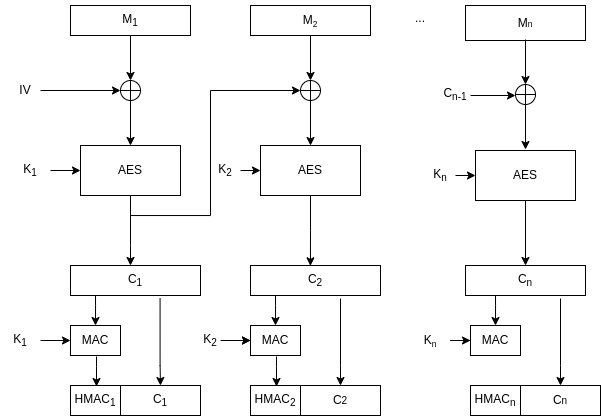
\includegraphics[width=250px]{chapters/res/chapter-3/img/encrypt.png}
  \caption{Enkripsi pesan secara dinamis untuk pesan yang dikirimkan dari Alice menuju Bob} \label{fig:solution.encrypt}
\end{figure}

\begin{figure}[!h]
  \centering
  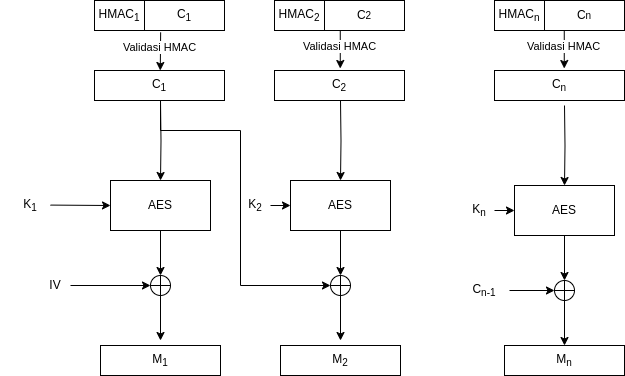
\includegraphics[width=250px]{chapters/res/chapter-3/img/decrypt.png}
  \caption{Dekripsi dan validasi pesan secara dinamis untuk pesan yang dikirimkan dari Alice menuju Bob} \label{fig:solution.decrypt}
\end{figure}

Pada proses awal komunikasi, akan dibentuk dua buah sistem \emph{chaos} melalui mekanisme pertukaran kunci \emph{diffie-hellman}. Kedua belah pihak akan melakukan pertukaran kunci memanfaatkan \emph{Diffie-Hellman}. Nilai hasil pertukaran kunci akan digunakan sebagai parameter awal nilai $(X_1, Y_1, Z_1)$ untuk sistem $S_1$ dan $(A_1, B_1, C_1)$ pada sistem chaos $S_2$. Hal ini dapat diperoleh dengan melakukan \emph{sclicing} bit hasil pertukaran kunci. Parameter $(X_1, Y_1, Z_1)$ dan $(A_1, B_1, C_1)$ bersifat rahasia. Penentuan nilai $IV$ akan ditentukan oleh pengirim pesan. Nilai ini akan dibuat secara acak memanfaatkan \emph{secure random} yang disediakan pada sistem operasi. Nilai $IV$  tidak bersifat rahasia.

Saat proses pertukaran kunci berhasil dan sistem \emph{chaos} berhasil dibuat, proses komunikasi akan dimulai. Misalkan, terdapat dua pihak yang melakukan komunikasi, yaitu Alice dan Bob. Sistem \emph{chaos} $S_1$ akan digunakan saat pengiriman data berlangsung dari Alice menuju Bob.  Sebaliknya, sistem \emph{chaos} $S_2$ akan digunakan saat pengiriman data berlangsung dari Bob menuju Alice.

Misalkan, pengriman data berlangsung dari Alice menuju Bob. Alice akan mengenkripsi blok $M_i$ menggunakan nilai $K_i$. Nilai $K_i$ dihasilkan berdasarkan hasil konversi nilai $X_i$ pada sistem $S_1$ menjadi bilangan bulat melalui fungsi $f$. Setelah pesan dienkripsi menjadi $C_i$, akan dihitung nilai MAC dengan kunci $K_i$ untuk $C_i$ dan disematkan pada $C_i$. Proses enkripsi berlangsung sebagaimana gambar \ref{fig:solution.encrypt}. Nilai $(X_{i+1}, Y_{i+1}, Z_{i+1})$ pada Alice akan dihitung apabila pesan $M_i$ berhasil dienkripsi menjadi $C_i$.  

Saat bob menerima pesan, bob akan memeriksa keabsahan data melalui MAC. Bob akan menghitung nilai $(X_i, Y_i, Z_i)$ dan membantuk nilai $K_i$. Setelah itu, Bob akan menghitung MAC $C_i$ dan membandingkannya dengan nilai MAC yang dikirimkan oleh Alice. Apabila nilai MAC sama, nilai $(X_{i-1}, Y_{i-1}, Z_{i-1})$ akan dihapus pada Bob. Selanjutnya, proses dekripsi dilakukan sebagaimana yang dijelaskan pada gambar \ref{fig:solution.decrypt}.
